\section{Algoritmo de traduccion de experimentos}

Como mencionamos en la seccion 9 un programa almacenable y ejecutable por el PP2 es una secuencia de 
instrucciones \(I_{1} ... I_{N}\) con \(1 < N < 512 \).
\\
Las instrucciones disponibles son:

\begin{itemize}
    \item Continue
    \item Loop
    \item Retl
    \item End
\end{itemize}

\noindent
No todos los programas escritos con estas instrucciones son admitidos como validos para el PP2, 
por esto tenemos las siguientes reglas:

\begin{itemize}
\item Regla 1: la instruccion End siempre es la ultima instruccion.
\item Regla 2: la intruccion End aparece solo una vez.
\item Regla 3: la intruccion End siempre esta presente.
\item Regla 4: un bucle siempre inicia con instruccion Loop y finaliza con Retl.
\item Regla 5: puede haber hasta 3 loops dentro de un loop.
\item Regla 6: la longitud del programa no puede ser mayor a 512 instrucciones.
\end{itemize}


\begin{figure}[!htb].
    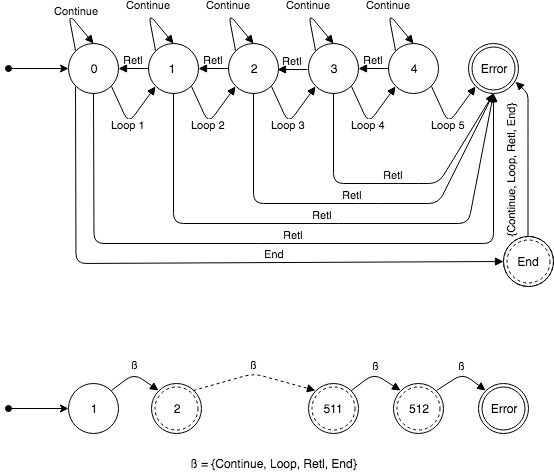
\includegraphics[width=\linewidth]{../figures/d12.jpg}
    \caption{Los programas aceptados por el PP2.}
    \label{fig:d12}
\end{figure}
 
\newpage
\begin{algorithm}
    \caption{Algoritmo de traduccion base}\label{euclid}
    \begin{algorithmic}[1]
    \Procedure{Translate}{P, L=0, S=[]}
    \State $ins \gets pop(P)$

    \If {$ins = Continue$}
    \State S.append(ins)
    \EndIf

    \If {$ins = Retl$}
        \If {$L > 0$}
            \State $S.append(\textit{ins})$
            \State $L \gets L-1$
            \State $Translate(P, L, S)$
        \Else
            \State \Return $error$
        \EndIf
    \EndIf
    
    \If {$ins = Loop$}
        \If {$L < 4$}
            \State $S.append(\textit{ins})$
            \State $L \gets L+1$
            \State $Translate(P, L, S)$
        \Else
            \State \Return $error$
        \EndIf
    \EndIf

    \If {$ins = End$}
        \If {$len(P) = 0$}
            \State $S.append(\textit{ins})$
        \Else
            \State \Return $error$
        \EndIf
    \EndIf

    \State \Assert{$ 0 < len(S) < 512$}
    \State \Return $S$
    \EndProcedure
    \end{algorithmic}
    \end{algorithm}
    
% traslate(P, L, S)

%     ins = next(P)

%     if ins = Continue:
%         S.append(ins)

%     if ins = Retl:
%         if(L!=0):
%             S.append(ins)
%             L--
%         else:
%             ret Error

%     if ins = Loop:
%         if(L<4):
%             S.append(ins)
%             L++
%         else:
%             ret Error
    
%     ret S

\newpage